\documentclass{beamer}
%
% Choose how your presentation looks.
%
% For more themes, color themes and font themes, see:
% http://deic.uab.es/~iblanes/beamer_gallery/index_by_theme.html
%
\mode<presentation>
{
  \usetheme{default}      % or try Darmstadt, Madrid, Warsaw, ...
  \usecolortheme{default} % or try albatross, beaver, crane, ...
  \usefonttheme{default}  % or try serif, structurebold, ...
  \setbeamertemplate{navigation symbols}{}
  \setbeamertemplate{caption}[numbered]
} 

\usepackage[english]{babel}
\usepackage[utf8]{inputenc}
\usepackage[T1]{fontenc}
\usepackage{amsmath,esint,textcomp,hyperref,graphicx,geometry,natbib,caption,subcaption,tikz,circuitikz}
\title[Semiconductor Solver]{Semiconductor Solver}
\author{Gaurav Somani}
\institute{CeNSE, IISc}
%\date{1 July,2020}

\begin{document}

\begin{frame}
  \titlepage
\end{frame}

% Uncomment these lines for an automatically generated outline.
%\begin{frame}{Outline}
%  \tableofcontents
%\end{frame}

\section{Introduction}

\begin{frame}{Introduction}

\begin{itemize}
  \item Like most of the physical systems, semiconductor system variables can be tied in a set of partial differential equations	  
  \item Due to non-linearity of equations, space variation of electric potential and current-voltage relationship in semiconductors is non-linear
  \item Can't apply ohm's law
  \item Analytical approximations can't always be made justifiably
  \item Numerical methods come to the rescue 
\end{itemize}

\end{frame}

\section{Fundamental Equations}

\subsection{Equilibrium}


\begin{frame}{Fundamental Equations:Equilibrium}

Equilibrium implies no electric current flow and constant fermi level.

\textbf{Poisson equation:}
\begin{equation}
\nabla^2 \psi = -\frac{q(N_D - N_A + p - n)}{\epsilon} \tag{1} \label{eq:1}
\end{equation} 

\textbf{Carrier Statistics:}
\begin{align*}
n = N_C F_{1/2}\left(\frac{q(\psi-\psi_i)}{k_BT}\right) \\
p = N_V F_{1/2}\left(\frac{-q(E_g+\psi-\psi_i)}{k_BT}\right) \tag{2} \label{eq:2}
\end{align*}

where $F_j$ represents complete Fermi-Dirac integral of order $j$

% Commands to include a figure:
%\begin{figure}
%\includegraphics[width=\textwidth]{your-figure's-file-name}
%\caption{\label{fig:your-figure}Caption goes here.}
%\end{figure}
\end{frame}

\subsection{Non-equilibrium steady state}

\begin{frame}{Fundamental Equations:Non-equilibrium steady state}

\textbf{Conservation equation:}
Recombination rate is rate at which carriers combine per unit volume per unit time.
\begin{equation}
R - G =  \frac{\vec{\nabla}.\vec{J_n}}{q} =-\frac{\vec{\nabla}.\vec{J_p}}{q}   \tag{3} \label{eq:3}
\end{equation}

\textbf{Drift-Diffusion:}
\begin{align*}
\vec{J_n} = -qn\mu_n\nabla\phi_n \\ 
\vec{J_p} = -qn\mu_p\nabla\phi_p  \tag{4} \label{eq:4}
\end{align*}

\textbf{SRH Recombination}:
\begin{align*}
R = \frac{pn - n_i^2}{\tau_n(p + n_i) + \tau_p(n + n_i)} \tag{5}\label{eq:5}
\end{align*}

G is generation rate (generally, due to optical excitation)

\end{frame}

\subsection{Geometry}
\begin{frame}{Domain geometry}
\begin{itemize}
	\item 2-D Cylindrically symmetric (r and z)
	\item 2-D Rectangular with reflection symmetry (x and y)
	\item 1-D (Rectangular) (x)
	\item 1-D (Circular) (r)
	\item 1-D (Spherical) (r)
\end{itemize}
\end{frame}	

\subsection{Boundary conditions}

\begin{frame}{Boundary conditions for well-defined solution}
\begin{itemize}
  \item Equilibrium : Potential boundary conditions and normal electric field boundary lead to unique solution for poisson equation	  
  \item Non-equilibrium steady state : Dirichlet boundary conditions are physically known (voltage bias and contact nature)
  \item Vertical boundaries have reflecting boundary conditions
\end{itemize}
\end{frame}

\subsection{Normalisation}

\begin{frame}{Normalisation}
\begin{itemize}
  \item Conversion of physical quantities to dimensionless form by dividing by suitable physical values\\
		\begin{align*}
		V_T = \frac{k_BT}{q}; L_D = \sqrt{\frac{\epsilon V_T}{q n_i}} \\
		E_0 = \frac{V_T}{L_D} ; J_o = \frac{q \mu_n n_i V_T}{L_D} \\
		t_0 = \frac{\epsilon}{q \mu_n n_i} ; R_o = \frac{n_i}{t_0}
		\tag{6} \label{eq:21} 
		\end{align*}
  		Leads to much simpler equations
\end{itemize}
\end{frame}
  		
\subsection{Linearisation and Discretisation}  		
\begin{frame}{Linearisation and Discretisation}
\begin{itemize}
  \item Linearisation : Linearisation of non-linear PDE about current solution \\
  		Non-linearity in poisson equation due to carrier statistics linearised using derivative wrt potential
  		\begin{align*}
		\nabla^2 \psi = r + \psi ( N_C F_{-1/2}(\bar{\Phi}-\psi_i) + N_V F_{-1/2}(\psi_i-E_g-\bar{\Phi}))
		\tag{7} \label{eq:39}
		\end{align*}
		where $\psi$ is the change in the potential approximation	  
  \item Discretisation : Discretisation of linearised PDE to set of linear equations \\
  		For poisson equation, discretised laplacian is used for different geometries\\
  		For conservative quantities, numerically integration over control area about each mesh point is performed.  	 
  \item Linearised equations when discretised lead to matrix equations  	
\end{itemize}
\end{frame}

\subsection{Implementation}
\begin{frame}{Input for equilibrium}
\begin{itemize}
	\item Set up mesh and contact nature (boundary conditions)
	\item Define doping profile
	\item Solve for equilibrium potential and carrier density
	\item Plot results	
\end{itemize}
\end{frame}

\begin{frame}{Input for biased system}
\begin{itemize}
	\item Set up mesh and contact nature (boundary conditions)
	\item Define doping profile and carrier lifetimes
	\item Define generation rate (default is 0 everywhere)
	\item Set bias sweep range
	\item Solve for potential, carrier density and current density
	\item Plot results
\end{itemize}
\end{frame}

\subsection{Mesh and boundary conditions}

\begin{frame}{Setting up mesh and boundary conditions}
\begin{itemize}
  \item Mesh generation : User inputs the critical points and mesh spacing. Automated non-uniform smooth mesh is generated by geometric interpolation. Mesh spacing should be less than $L_D$ (debye length) to resolve fine features. Also, non-uniform mesh allows having good condition number. Mesh should be fine at junctions.
  \item Boundary conditions : Electrical boundary conditions in user input converted to physical boundary conditions in terms of solution variables
\end{itemize}
\end{frame}

\subsection{Initial Guess}
\begin{frame}{Initial guess}
\begin{itemize}
	\item \textbf{Equilibrium Poisson Equation}: Based on analytical solution after removing coupling between neighbouring mesh points \\
		Based on the reasoning that device can be constructed by putting pieces of semiconductor together
	\item \textbf{Biased non-equilibrium steady state}: For initial bias, solution at equilibrium is used as initial guess 
\end{itemize}  
\end{frame}

\subsection{Numerical methods}

\begin{frame}{Numerical methods}
\begin{itemize}
  \item Gauss-Laguerre quadrature for numerical evaluation of FD integral
  	\begin{align*}
	F_j(x) =  \frac{1}{\Gamma(j+1)} \int^\infty_0 w_j(t)\frac{1}{e^{-t}+e^{-x}} dt \\= \frac{1}{\Gamma(j+1)} \int^\infty_0 w_j(t)g(t) dt \\
	where\ w_j(t) = t^j e^{-t}\ and\  g(t) = \frac{1}{e^{-t}+e^{-x}}.
	\end{align*}
  
  \item SOR + Multi-grid
  \item Alternate direction implicit method
  \item Tridiagonal matrix algorithm
  \item Relaxation method
  \item Newton-Raphson method
  \item Banded matrix algorithms
\end{itemize}
\end{frame}

\subsection{SOR + multigrid}
\begin{frame}{SOR + multigrid}
\begin{itemize}
	\item SOR (iterative method) is used for equilibrium calculation as good initial guess is available
	\item Potential has low frequency modes
	\item SOR on fine mesh (more points) takes a large number of iterations to resolve   
	\item SOR with multi-grid resolves lower frequency modes at coarser mesh
	\item Mesh is coarsened recursively until mesh becomes coarse enough so solution becomes computationally cheap 
	\item Solution at coarser mesh is interpolated to finer mesh as initial guess
\end{itemize}  
\end{frame}

\subsection{ADI}
\begin{frame}{ADI}
\begin{itemize}
	\item 1D problem leads to tridiagonal matrix with fast solution 
	\item ADI by splitting the laplacian along orthogonal dimensions
	\item Faster than SOR + multigrid in most cases
\end{itemize}  
\end{frame}

\subsection{Relaxation for coupled PDE at steady state}
\begin{frame}{Relaxation for coupled PDE at steady state}
\begin{itemize}
	\item Coupled PDE system solved by solving one PDE at a time considering only one solution variable
	\item Robust for low bias and insensitive to poor guess
	\item Slow(linear) convergence
\end{itemize}  
\end{frame}

\subsection{Newton's method for coupled PDE}
\begin{frame}{Newton's method for coupled PDE}
\begin{itemize}
	\item Linearised description of coupled PDE system in terms of 3N variables is calculated  
	\item Newton's method is applied to Jacobian to calculate next approximate solution 
	\item Fast(Quadratic) convergence
	\item Highly sensitive to initial guess
	\item Used in combination with relaxation method to ensure robustness and speed 
\end{itemize}  
\end{frame}

\subsection{Optimisations}
\begin{frame}{Faster implementation}
\begin{itemize}
  \item Red-black scheme of ordering variables for vectorized implementation of SOR
  \item Pre-computation of Fermi-Dirac integral and use of cubic splines to approximate it at runtime
  \item Alternate row and alternate column iterations for vectorized ADI 
  \item Reordering of variables of coupled PDE for steady state to form banded matrix
  \item Combination of relaxation and newton-raphson methods
  \item Pre-computation of Laplacian stencil 
\end{itemize}
\end{frame}

\subsection{Numerical issues}
\begin{frame}{Problems related to numerical solution}
\begin{itemize}
\item Noisy current density\\ 
\textbf{Solution} : Under steady state reverse bias, currents become very low and exponent calculation of very close numbers lead to loss of numerical precision. So, instead of 64 bits float, 80 bits long double is used. It makes solution reliable and can speed up convergence in most cases.

\item High coupling between coupled PDE at high bias under steady state leading to non-convergence or very slow convergence\\
\textbf{Solution} : Jacobian of coupled system is used to linearise the system. Then, newton-raphson method is applied to linearised system in $3N$ variables with reordered variables leading to banded matrix which speeds up the convergence
 
\end{itemize}
\end{frame}

\section{Results}

\begin{frame}
\begin{figure}[h!]
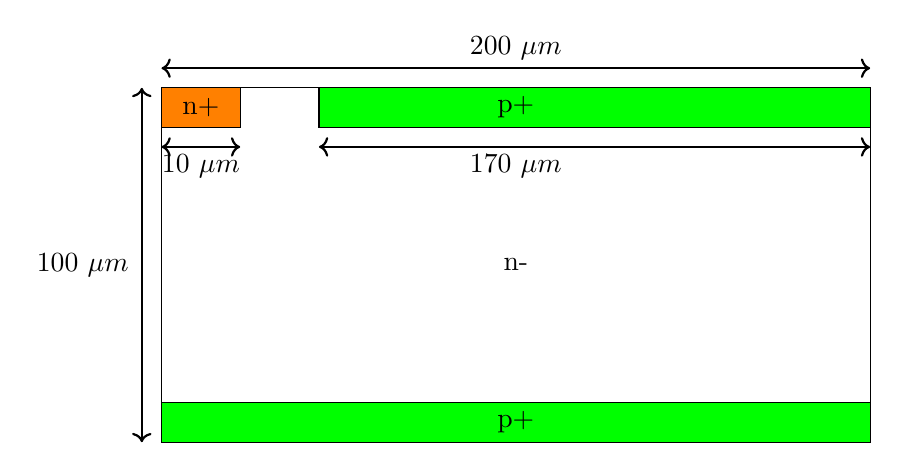
\begin{tikzpicture}
\def \thickness {4.5}
\def \width {9}
\draw [thick, <->] (-0.25,\thickness) -- (-0.25,0);
\draw [thick, <->] (0,\thickness+0.25) -- (\width,\thickness+0.25);
\draw [thick, <->] (2,\thickness-0.75) -- (\width,\thickness-0.75);
\node at (-1,0.5*\thickness) {100 $\mu m$};
\node at (0.5*\width,\thickness+0.5) {200 $\mu m$};
\node at (0.5*\width,\thickness-1) {170 $\mu m$};
\draw (0,0) rectangle (\width,\thickness);
\draw[fill=orange] (0,\thickness) rectangle (1,\thickness-0.5);
\draw [thick, <->] (0,\thickness-0.75) -- (1,\thickness-0.75);
\node at (0.5,\thickness-0.25) {n+};
\node at (0.5,\thickness-1) {10 $\mu m$};
\draw[fill=green] (2,\thickness-0.5) rectangle (\width,\thickness);
\node at (0.5*\width,\thickness-0.25) {p+};	
\draw[fill=green] (0,0) rectangle (\width,0.5);
\node at (0.5*\width,0.25) {p+};	
\node at (0.5*\width,0.5*\thickness) {n-};
\end{tikzpicture}
\caption{Input structure (SDD)}
\label{fig:SDD}
\end{figure}
\end{frame}

\begin{frame}
\begin{figure}[h!]
     \centering
        \includegraphics[width=\textwidth]{equilibrium_potential_2d.png}
         \caption{Potential contour plot showing potential variation near the junction by this solver}
         \label{fig:pot_2d}
     \end{figure}
\end{frame}
%
%\begin{frame}
%\begin{figure}[h!]
%     \centering
%        \includegraphics[width=\textwidth]{equilibrium_holes_2d.png}
%         \caption{Hole density contour plot showing depletion near the junction}
%         \label{fig:hole_2d}
%     \end{figure}
%\end{frame}

%\begin{frame}
%\begin{figure}[h!]
%     \centering
%        \includegraphics[width=\textwidth]{potential.png}
%         \caption{Potential contour plot by commercial solver}
%         \label{fig:pot_comm}
%     \end{figure}
%\end{frame}

%\begin{frame}
%\begin{figure}[h!]
%     \centering
%        \includegraphics[width=\textwidth]{equilibrium_electrons_2d.png}
%         \caption{Electron density contour plot showing depletion near the junction}
%         \label{fig:electron_2d}
%     \end{figure}
%\end{frame}
%
\begin{frame}
Commercial simulator used to compare results is SILVACO ATLAS.
\begin{figure}[h!]
     \centering
        \includegraphics[width=\textwidth]{comparision.png}
         \caption{Potential section at $r=41.2 \mu m$}
         \label{fig:pot_sec}
     \end{figure}
\end{frame}

\begin{frame}
\begin{figure}[h!]
\centering
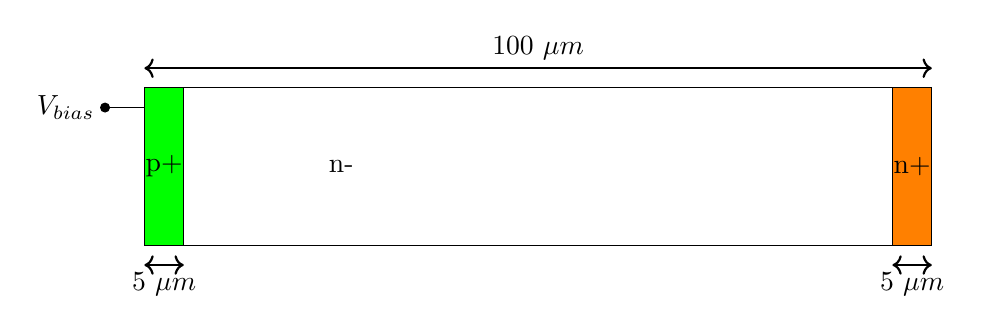
\begin{tikzpicture}
\def \thickness {2}
\def \width {10}
\draw [thick, <->] (0,\thickness+0.25) -- (\width,\thickness+0.25);
\draw [thick, <->] (0,-0.25) -- (0.5,-0.25);
\draw [thick, <->] (\width-0.5,-0.25) -- (\width,-0.25);
\node at (\width-0.25,-0.5) {5 $\mu m$};
\node at (0.25,-0.5) {5 $\mu m$};
\node at (0.5*\width,\thickness+0.5) {100 $\mu m$};
\draw [short, *-] (-0.5,\thickness-0.25) to (0,\thickness-0.25);  
\node at (-1,\thickness-0.25) {$V_{bias}$};  
\draw (0,0) rectangle (\width,\thickness);
\draw[fill=green] (0,0) rectangle (0.5,\thickness);
\node at (0.25,0.5*\thickness) {p+};
\draw[fill=orange] (\width-0.5,0) rectangle (\width,\thickness);
\node at (\width-0.25,0.5*\thickness) {n+};
\node at (0.25*\width,0.5*\thickness) {n-};
\end{tikzpicture}
\caption{PIN diode}
\label{fig:PIN}
\end{figure}
\end{frame}

\subsection{Potential and current density in a biased p-n junction}

\begin{frame}{Results : Potential at equilibrium}
\begin{figure}[h!]
     \centering
        \includegraphics[width=0.8\textwidth,height=5cm]{comparision_pin.png}
         \caption{Potential barrier at equilibrium}
         \label{fig:pot_eq}
     \end{figure}
\begin{align*}
W_{dep} = \sqrt{\frac{2\epsilon_{Si} V_{bi}}{q N}} 
\end{align*}
which is about $25 \mu m$      
\end{frame}

\begin{frame}{Results : Potential in a biased pn-junction}
\begin{figure}[h!]
     \centering
        \includegraphics[width=0.8\textwidth]{comparision_pin_fb.png}
         \caption{Potential barrier lowered in forward bias}
         \label{fig:pot_fb}
     \end{figure}
\end{frame}
     
\begin{frame}   
\begin{figure}[h!]
     \centering
        \includegraphics[width=0.8\textwidth]{comparision_pin_rb.png}
         \caption{Potential barrier increased in reverse bias}
         \label{fig:pot_rb}
     \end{figure}     

\end{frame}

\begin{frame}{Results: Current density in a biased p-njunction}
Current density for an ideal p-n junction diode can be approximated by :
\begin{align*}
J = J_0 (e^{qV/k_BT}-1) 
\end{align*}

\begin{figure}[h!]
     \centering
        \includegraphics[width=0.8\textwidth]{forward_bias.png}
         \caption{Current density in forward bias(Linear scale)}
         \label{fig:jv}
     \end{figure}

\end{frame}

\begin{frame}{Results: Current density in a biased pn-junction}

\begin{figure}[h!]
     \centering
        \includegraphics[width=0.8\textwidth]{jv_diode_log.png}
         \caption{Current density in forward bias(Logarithmic scale) (compare with \ref{fig:jv_bart})}
		 \label{fig:jvl}     
     \end{figure}

\end{frame}

\begin{frame}
\begin{figure}[h!]
     \centering
        \includegraphics[width=0.8\textwidth]{bart.png}
         \caption{Image taken from Principles of Semiconductor Devices,B. Van Zeghbroeck, 2011}
		 \label{fig:jv_bart}     
     \end{figure}
\end{frame}


\begin{frame}

\begin{align*}
J_{gen} = q n_i \frac{W_D}{\tau_n + \tau_p} \approx 10^{-8} A/cm^2
\end{align*}


\begin{figure}[h!]
     \centering
        \includegraphics[width=0.7\textwidth]{reverse_bias.png}
         \caption{Current density in reverse biased PIN diode due to generation happening in depletion region (See noisy current density with commercial simulator due to lower precision of 64 bits compared to 80 bits used in this solver)}
		 \label{fig:jvr}     
     \end{figure}         
\end{frame}

\end{document}
